Having explored existing data models and tested their limitations against several case studies from the Middle Ages, we propose a model with the entities and relationships represented in Figure \ref{fig:ProposedEntities}. To begin, we present all the entities we believe necessary for a data model tasked with organizing and delivering information about texts and traditions in Medieval literature, particularly texts about chivalric tales and legends. Then, we list all the attributes each entity features. Compared to the former, this latter section is more likely to need further modifications based on the idiosyncratic qualities of different literary corpora.

\subsection{Intertextuality}

On the top level of Figure \ref{fig:ProposedEntities}, running from left to right, are the three abstract entities, \textit{Cycle}, \textit{Work}, and \textit{Text}, that manage information about intertextuality in our corpus. \textit{Works} and \textit{Cycles} can be nested together within the scope of a \textit{Cycle}, based on the \textit{Works'} narrative content; both entities have the attribute ``is part of,'' which points to a \textit{Cycle} entity. \textit{Works} can also be modeled on other works, as in the case of a new \textit{Work} compiling and reworking the episodes and characters from two or more pre-existing \textit{Works}. The data model also registers intertextuality amongst \textit{Texts}, which can be modeled on one another as translations, prosifications, abbreviations, elaborations, versifications, or other forms of adapting the expression (\textit{Text}) of a common \textit{Work}. The nature of a \textit{Text's} relationship to a model \textit{Text} can be inferred through differences and similarities in the two entities' attributes, such as their language and literary form.

\begin{figure}[httb!]
    \begin{center}
        \tikzstyle{s} = [rectangle, rounded corners, minimum width=2cm, text width=2cm, minimum height=1cm, text centered, draw=black]
\tikzstyle{arrow} = [thick,->,>=stealth]
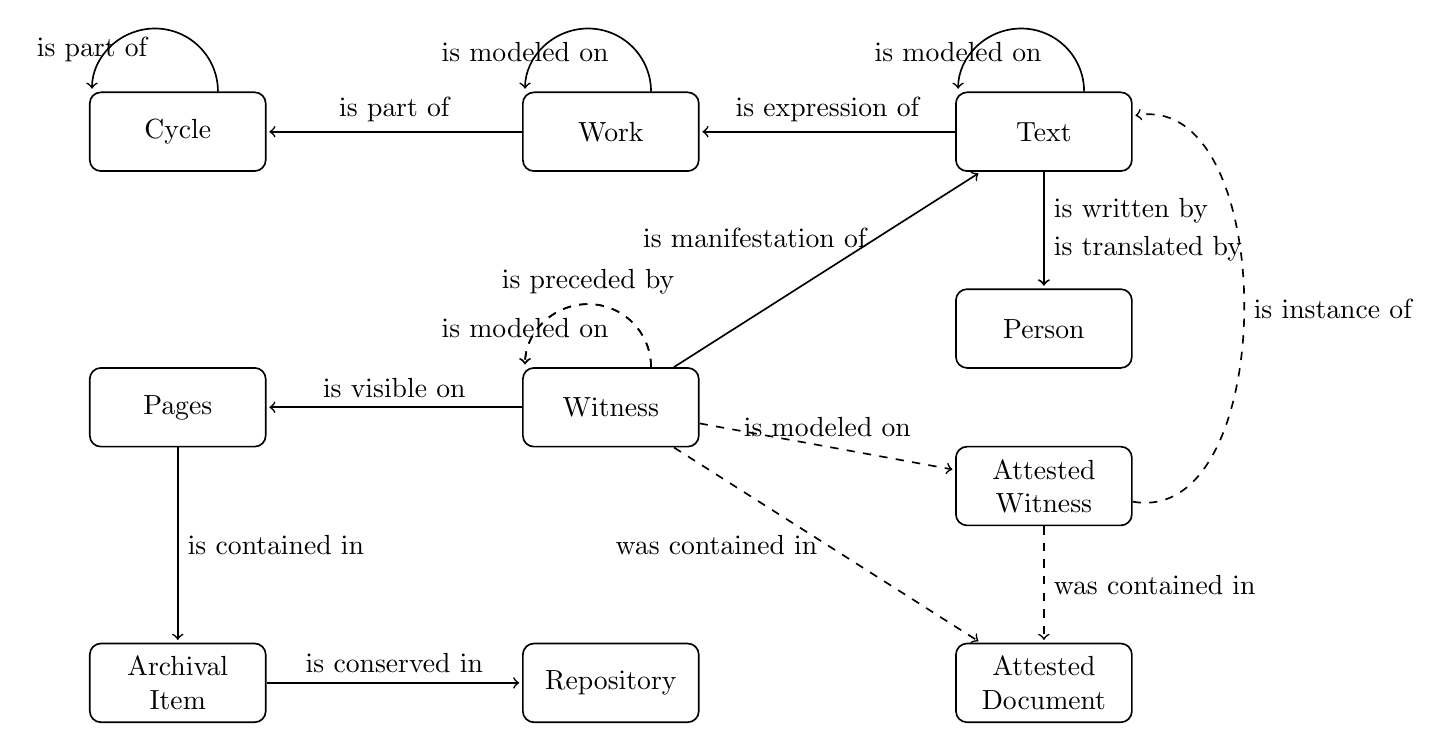
\begin{tikzpicture}[-,shorten >=1pt,auto,node distance=2.5cm,semithick]
\tikzstyle{every state}=[fill=red,draw=none,text=white]

\node[s] (cycle) [] {Cycle};
\node[s] (work) [right of=cycle, xshift=3cm] {Work};
\node[s] (text) [right of=work, xshift=3cm] {Text};

\node[s] (person) [below of=text] {Person};

\node[s] (attestedWitness) [below of=person, yshift=0.5cm] {Attested Witness};

\node[s] (witness) [below of=work, yshift=-1cm] {Witness};

\node[s] (pages) [left of=witness, xshift=-3cm] {Pages};

\node[s] (item) [below of=pages, yshift=-1cm] {Archival Item};

\node[s] (repo) [right of=item, xshift=3cm] {Repository};

\node[s] (document) [right of=repo, xshift=3cm] {Attested Document};

% \draw[dashed, ->] (witness.-45) arc (200:475:8mm) 
%   node[pos=0.5, below] () {is preceded by};
\draw[dashed, ->] (witness.45) arc (0:180:8mm)
  node[above, pos=0.5] () {is preceded by};
\draw[dashed, ->] (witness.45) arc (0:180:8mm)
  node[above, yshift=0.25cm] () {is modeled on};
\draw[->] (cycle.45) arc (0:180:8mm) 
  node[above, yshift=0.25cm] () {is part of};
\draw[->] (work.45) arc (0:180:8mm) 
  node[above, yshift=0.25cm] () {is modeled on};
\draw[->] (work) -- (cycle)
  node[pos=0.5, above] () {is part of};
\draw[->] (text) -- (work)
  node[pos=0.5, above] () {is expression of};
\draw[->] (witness) -- (text)
  node[pos=0.66, left] () {is manifestation of};
\draw[dashed,->] (witness) -- (document)
  node[pos=0.5, left] () {was contained in};
\draw[->] (pages) -- (item)
  node[pos=0.5, right] () {is contained in};
\draw[->] (witness) -- (pages)
  node[pos=0.5, above] () {is visible on};
\draw[->] (item) -- (repo)
  node[pos=0.5, above] () {is conserved in};
\draw[->] (text.45) arc (0:180:8mm) 
  node[yshift=0.25cm, above] () {is modeled on};
\draw[->] (text) -- (person)
  node[pos=0.66, right] {is translated by};
\draw[->] (text) -- (person)
  node[pos=0.33, right] {is written by};
\draw[dashed, ->] (witness) -- (attestedWitness)
  node[pos=0.5, above] {is modeled on};
\draw[dashed, ->] (attestedWitness) -- (document)
  node[pos=0.5, right] {was contained in};

\path[every node]
  (attestedWitness) edge[dashed, ->, bend right=100] node [pos=0.5, right] {is instance of} (text)
  ;

\end{tikzpicture}
    \end{center}
\caption{Proposed Entities.}
\label{fig:ProposedEntities}
\end{figure}

\subsection{Archival Evidence}

Stemming from an extant \textit{Witness} are potentially four types of relationships to other entities. First and foremost, a \textit{Witness} must relate to one and only one \textit{Text}. By definition, a \textit{Witness} is an extant version of a \textit{Text's} linguistic content, spelled out in a sequence of characters, as demonstrated in Table \ref{tab:TextVersions}. Therefore, the \textit{Witness} must be the manifestation of a \textit{Text}. Second, the \textit{Witness}, by virtue of being extant, must be visible on the \textit{Pages} of an \textit{Archival Item}. When the version of a \textit{Text} has survived through fragments, one of the fragmented version's \textit{Witnesses} can relate to another fragment through the attribute ``is preceded by.'' An example of this inter-\textit{Witness} relationship is demonstrated in the case of the \textit{Chanson d'Aspremont} and the Table \ref{tab:CampsAspremont}. Finally, a \textit{Witness} can have formerly been contained in a document which has not survived but to whose historical existence scholars attest based on philological and codicological evidence.

\textit{Pages} represents an uninterrupted set of folios and, when digitized, images of an \textit{Archival Item} on which the text content of a \textit{Witness} can be read. In our data model, a \textit{Pages} entity, which depends on an extant \textit{Witness}, must be contained in an \textit{Archival Item}. The \textit{Archival Item} can relate to multiple \textit{Pages} entities. However, the first folio of one \textit{Pages} entity must not come before the last folio of another \textit{Pages} entity in the same \textit{Archival Item}. In other words, \textit{Pages} entities cannot overlap. They represent a unique set of leafs or pages in an \textit{Archival Item}, and they present the content of only one \textit{Witness}. Lastly, the \textit{Archival Item}, being an object one can consult and which continues to persist, contrary to the \textit{Attested Document}, must be conserved in a \textit{Repository}.

\subsection{Genealogy of a \textit{Text}}
\label{sub:Graph}

While the proposed data model manages metadata about intertextuality within the corpus, its relational framework does not register how \textit{Witnesses} derive from one another. This choice reflects an assumption about intertextuality, meaning \textit{Works'} and \textit{Texts'} models, and stemma, meaning \textit{Witness'} models. On the one hand, we assume a relatively consistent consensus has been reached on the models of \textit{Works} and \textit{Texts}. We presume scholars and archivists have largely accepted as historical fact the assertion that one \textit{Text} is a translation of another \textit{Text}, that a \textit{Work} is a compilation of other \textit{Works}, that one \textit{Text} is the prose version of another \textit{Text}, and so on. Through analyses of the content and literary form of extant \textit{Witnesses} that are examples of \textit{Texts} and \textit{Works}, such claims of genealogy and intertextuality tend not to attract as much skepticism as claims scholars posit about which scribe derived their \textit{Witness} (Sahle's text-as-version) from the example of an older \textit{Witness}.

Such stemmatological claims are crucial, and we want to model them for the corpus. However, in addition to establishing a relationship between two \textit{Witness} entities, it is also critical to cite the source of that attested dependence. Furthermore, we want to permit conflicting stemma without over complicating the model's relationships. While it is possible to model such connections in a relational framework, exploiting those connections to respond to users' queries risks pushing the model to become over complex. The choice becomes one between exploting one over-complicated model or harmonizing and jointly exploiting two simpler models.

Rather than reinvent the wheel and model stemma in a complex relational framework, we propose pairing the former with a graph framework, which philologists have used for decades.\footcite[][]{Zundert2020} The relational framework's main tasks are, therefore, to generate entities relevant to our corpus, store metadata about them, and establish intertextual relations at the level of the abstract, narrative content, meaning the \textit{Work} and \textit{Text}. In conjunction, the graph database's \textit{Witness} nodes will bear the same identifier as their counterpart in the relational database and thus can be enriched with metadata.

The project \textit{OpenStemmata} has already designed a workflow through which contributors can encode stemma that have been published in a scholarly context or otherwise submitted by scholars. For example, Giovanni Palumbo and Paolo Rinoldi, who, while developing a critical edition of the French \textit{Chanson d'Aspremont}, produced a stemma of the first part of the \textit{Text}. Their stemma was encoded and uploaded to the \textit{OpenStemmata} database, and we have represented it here in Figure \ref{fig:GraphFramework}. The graph's gray node P\textsubscript{4} is equivalent to the \textit{Witness} P\textsubscript{4} in our earlier \textit{Chanson d'Aspremont} test case, as seen in Figures \ref{fig:BNFNAF5094}, \ref{fig:AspremontCFBNF}, and \ref{fig:WitnessRelations}.

\begin{figure}[htb!]
    \begin{center}
        \tikzstyle{s} = [circle, minimum width=1cm, text width=1cm, minimum height=1cm, text centered, draw=black]
\tikzstyle{n} = [circle, minimum width=1cm, text width=1cm, minimum height=1cm, text centered, draw=black, fill=gray!30]
\tikzstyle{p} = [circle, minimum width=1cm, text width=1cm, minimum height=1cm, text centered, draw=black, line width=0.75mm, fill=gray!30]
\tikzstyle{arrow} = [thick,->,>=stealth]
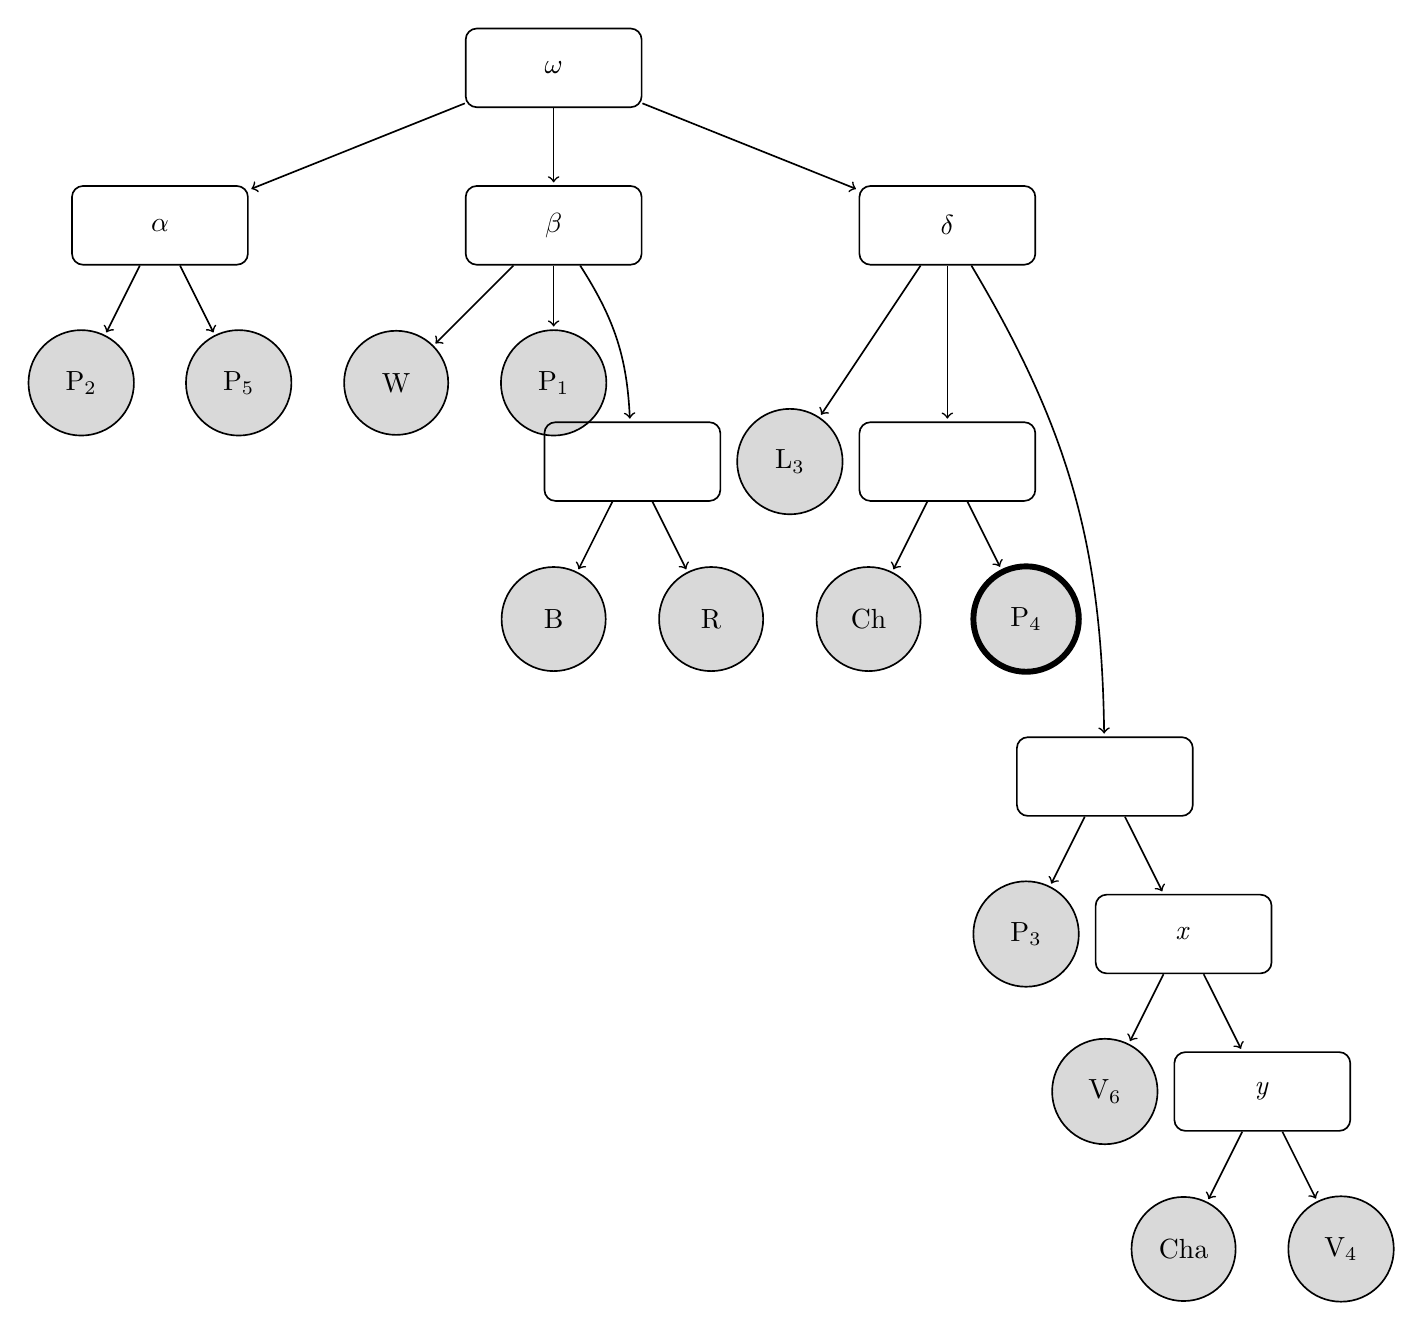
\begin{tikzpicture}[-,shorten >=1pt,auto,node distance=2cm,semithick]
\tikzstyle{every state}=[fill=red,draw=none,text=white]

\node[s] (w) {$\omega$};

\node[s] (a) [below of=w, xshift=-5cm] {$\alpha$};
\node[n] (p2) [below of=a, xshift=-1cm] {P\textsubscript{2}};
\node[n] (p5) [below of=a, xshift=1cm] {P\textsubscript{5}};

\path[every node/.style={font=\sffamily\small}]
    (w) edge[->] node[]{} (a)
    (a) edge[->] node[]{} (p2)
    (a) edge[->] node[]{} (p5)
;

\node[s] (b) [below of=w] {$\beta$};
\node[n] (W) [below of=b, xshift=-2cm] {W};
\node[n] (p1) [below of=b] {P\textsubscript{1}};
\node[s] (bb) [below of=b, yshift=-1cm, xshift=1cm] {};
\node[n] (B) [below of=bb, xshift=-1cm] {B};
\node[n] (R) [below of=bb, xshift=1cm] {R};

\path[every node/.style={font=\sffamily\small}]
    (w) edge[->] node[]{} (b)
    (b) edge[->] node[]{} (W)
    (b) edge[->] node[]{} (p1)
    (b) edge[->, bend left=15] node[]{} (bb)
    (bb) edge[->] node[]{} (B)
    (bb) edge[->] node[]{} (R)
;

\node[s] (d) [below of=w, xshift=5cm] {$\delta$};
\node[n] (l3) [below of=d, yshift=-1cm, xshift=-2cm] {L\textsubscript{3}};
\node[s] (dd1) [right of=l3] {};
\node[n] (ch) [below of=dd1, xshift=-1cm] {Ch};
\node[p] (p4) [below of=dd1, xshift=1cm] {P\textsubscript{4}};
\node[s] (dd2) [below of=d, xshift=2cm, yshift=-5cm] {};
\node[n] (p3) [below of=dd2, xshift=-1cm] {P\textsubscript{3}};
\node[s] (x) [below of=dd2, xshift=1cm] {\textit{x}};
\node[n] (v6) [below of=x, xshift=-1cm] {V\textsubscript{6}};
\node[s] (y) [below of=x, xshift=1cm] {\textit{y}};
\node[n] (cha) [below of=y, xshift=-1cm] {Cha};
\node[n] (v4) [below of=y, xshift=1cm] {V\textsubscript{4}};

\path[every node/.style={font=\sffamily\small}]
    (w) edge[->] node[]{} (d)
    (d) edge[->] node[]{} (l3)
    (d) edge[->] node[]{} (dd1)
    (dd1) edge[->] node[]{} (ch)
    (dd1) edge[->] node[]{} (p4)
    (d) edge[->, bend left=15] node[]{} (dd2)
    (dd2) edge[->] node[]{} (p3)
    (dd2) edge[->] node[]{} (x)
    (x) edge[->] node[]{} (v6)
    (x) edge[->] node[]{} (y)
    (y) edge[->] node[]{} (cha)
    (y) edge[->] node[]{} (v4)
;

\end{tikzpicture}

% \node[s] (w) {$\omega$};
% \node[s] (wl) [below of=w, xshift=-2cm] {};
% \node[s] (a) [below of=w, xshift=2cm] {$\alpha$};
% \node[s] (b) [below of=wl, xshift=-4cm] {$\beta$};
% \node[s] (gamma) [below of=wl] {$\gamma$};
% \node[n] (W) [below of=b, xshift=-2cm] {W};
% \node[n] (p5) [below of=b] {P\textsubscript{5}};
% \node[s] (gammal) [below of=gamma] {};
% \node[n] (l3) [below of=gammal, xshift=-2cm] {L\textsubscript{3}};
% \node[n] (ch) [below of=gammal] {Ch};
% \node[s] (x) [below of=gamma, xshift=2cm] {\textit{x}};
% \node[s] (y) [below of=x] {\textit{x}};
% \node[n] (cha) [below of=y, xshift=-1cm] {Cha};
% \node[n] (v4) [below of=y, xshift=1cm] {V\textsubscript{4}};
% \node[n] (v6) [below of=x, xshift=2cm] {V\textsubscript{6}};
% \node[n] (p2) [below of=a] {P\textsubscript{2}};
% \node[n] (p3) [below of=a, xshift=2cm] {P\textsubscript{3}};
% \node[n] (l2) [below of=a, xshift=4cm] {L\textsubscript{2}};

% \path[every node/.style={font=\sffamily\small}]
%     (w) edge[->] node[]{} (a)
%     (w) edge[->] node[]{} (wl)
%     (wl) edge[->] node[]{} (b)
%     (wl) edge[->] node[]{} (gamma)
%     (b) edge[->] node[]{} (W)
%     (b) edge[->] node[]{} (p5)
%     (gamma) edge[->] node[]{} (gammal)
%     (gamma) edge[->] node[]{} (x)
%     (gammal) edge[->] node[]{} (l3)
%     (gammal) edge[->] node[]{} (ch)
%     (x) edge[->] node[]{} (y)
%     (x) edge[->] node[]{} (v6)
%     (y) edge[->] node[]{} (cha)
%     (y) edge[->] node[]{} (v4)
%     (a) edge[->] node[]{} (p2)
%     (a) edge[->] node[]{} (p3)
%     (a) edge[->] node[]{} (l2)
% ;

% \end{tikzpicture}
    \end{center}
\caption{Stemma of extant \textit{Witnesses} (gray) and supposed witnesses (white) of the first part of the French \textit{Chanson d'Aspremont} by G. Palumbo and P. Rinoldi.}
\label{fig:GraphFramework}
\end{figure}

We propose outsourcing the data model's \textit{Text} genealogies to the \textit{OpenStemmata} project's established workflow, encoding standards, and open-source repository. Subsequently, we reconcile the \textit{Witness} nodes in the \textit{OpenStemmata} database, further valorizing and enriching those publications, with records registered in our proposed relational data model. Finally, having linked the two record types, such as the \textit{Witness} P\textsubscript{4} of the Anglo-Norman \textit{Chanson d'Aspremont}, the data model can deliver thoroughly enriched and linked records based on users' requests.

\subsection{Reconciling and citing records}

Finally, we propose a \textit{Reference} table (see Figure \ref{fig:ProposedEntitiesReference}), which associates certain entities with bibliographic resources. This last addition serves two purposes. First, it associates an entity with a unique identifier in an authoritative aggregator, such as WikiData, Biblissima, and VIAF (Virtual International Authority File). This association helps reconcile potentially duplicate records in the data model and helps reconcile records between the relational data model and an \textit{OpenStemmata} graph. Second, \textit{Reference} associates entities with scholarly citations. In addition to making the data model interoperable with other databases, including VIAF, the \textit{Reference} entity also allows us to enrich records with a scholarly bibliography.

\begin{figure}[htb!]
    \begin{center}
        \tikzstyle{s} = [rectangle, rounded corners, minimum width=2cm, text width=2cm, minimum height=1cm, text centered, draw=black]
\tikzstyle{arrow} = [thick,->,>=stealth]
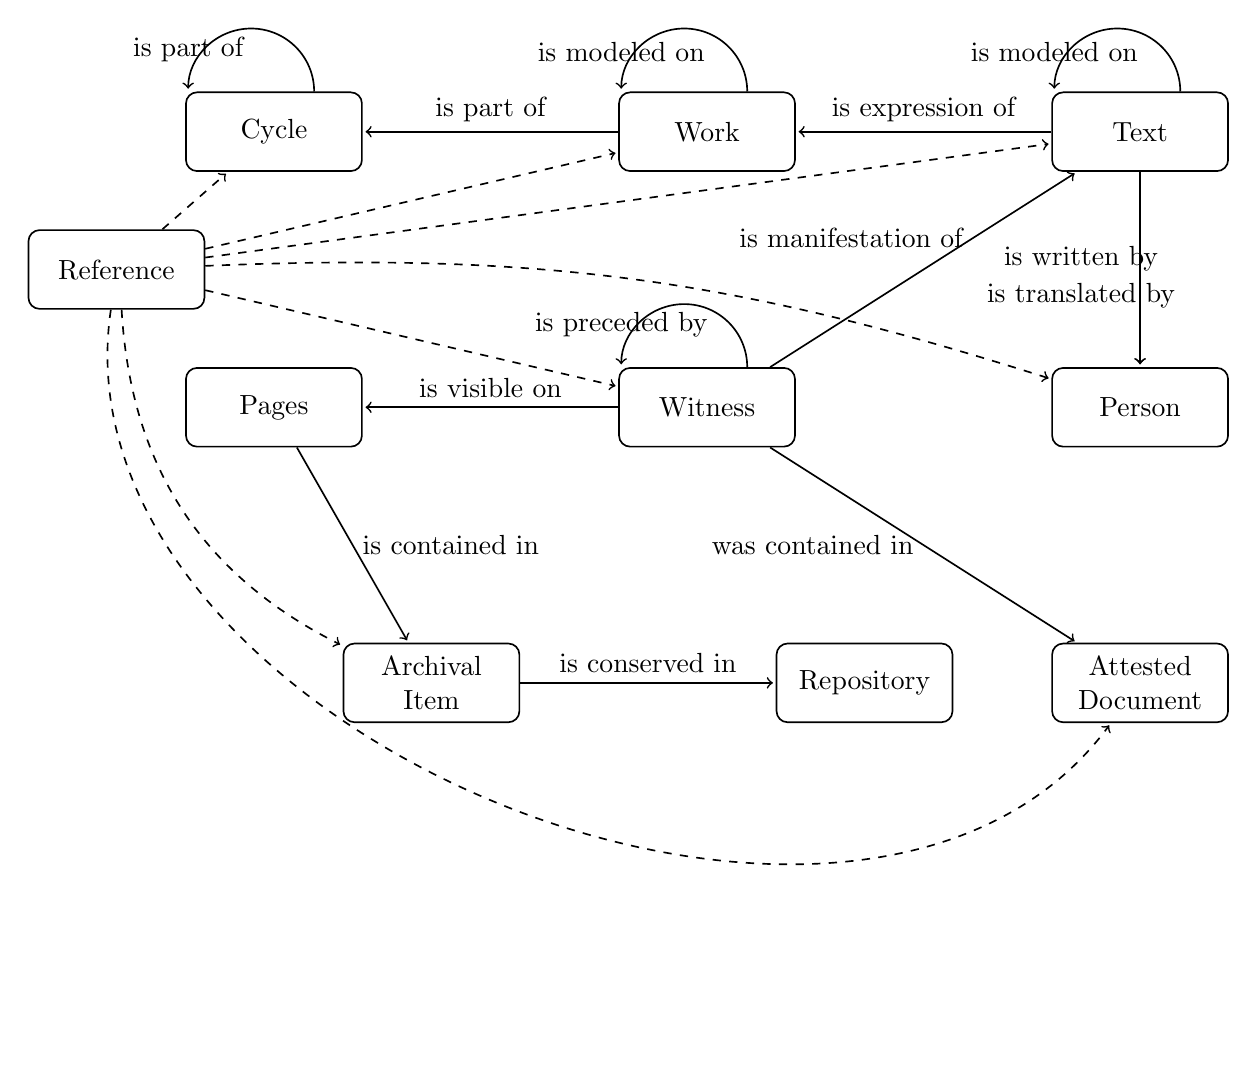
\begin{tikzpicture}[-,shorten >=1pt,auto,node distance=2.5cm,semithick]
\tikzstyle{every state}=[fill=red,draw=none,text=white]

\node[s] (cycle) [] {Cycle};
\node[s] (work) [right of=cycle, xshift=3cm] {Work};
\node[s] (text) [right of=work, xshift=3cm] {Text};

\node[s] (witness) [below of=work, yshift=-1cm] {Witness};

\node[s] (person) [right of=witness, xshift=3cm] {Person};

% \node[s] (attestedWitness) [below of=person, yshift=0.5cm] {Attested Witness};

\node[s] (pages) [left of=witness, xshift=-3cm] {Pages};

\node[s] (item) [below of=pages, yshift=-1cm, xshift=2cm] {Archival Item};

\node[s] (repo) [right of=item, xshift=3cm] {Repository};

\node[s] (document) [right of=repo, xshift=1cm] {Attested Document};

\node[s] (reference) [above of=pages, xshift=-2cm, yshift=-0.75cm] {Reference};

% \draw[dashed, ->] (witness.-45) arc (200:475:8mm) 
%   node[pos=0.5, below] () {is preceded by};
\draw[->] (witness.45) arc (0:180:8mm)
  node[above, yshift=0.25cm] () {is preceded by};
% \draw[dashed, ->] (witness.45) arc (0:180:8mm)
%   node[above, yshift=0.25cm] () {is modeled on};
\draw[->] (cycle.45) arc (0:180:8mm) 
  node[above, yshift=0.25cm] () {is part of};
\draw[->] (work.45) arc (0:180:8mm) 
  node[above, yshift=0.25cm] () {is modeled on};
\draw[->] (work) -- (cycle)
  node[pos=0.5, above] () {is part of};
\draw[->] (text) -- (work)
  node[pos=0.5, above] () {is expression of};
\draw[->] (witness) -- (text)
  node[pos=0.66, left] () {is manifestation of};
\draw[->] (witness) -- (document)
  node[pos=0.5, left] () {was contained in};
\draw[->] (pages) -- (item)
  node[pos=0.5, right] () {is contained in};
\draw[->] (witness) -- (pages)
  node[pos=0.5, above] () {is visible on};
\draw[->] (item) -- (repo)
  node[pos=0.5, above] () {is conserved in};
\draw[->] (text.45) arc (0:180:8mm) 
  node[yshift=0.25cm, above] () {is modeled on};
\draw[->] (text) -- (person)
  node[pos=0.75, above, xshift=-0.75cm] {is translated by};
\draw[->] (text) -- (person)
  node[pos=0.33, below, xshift=-0.75cm] {is written by};
% \draw[dashed, ->] (witness) -- (attestedWitness)
%   node[pos=0.5, above] {is modeled on};
% \draw[dashed, ->] (attestedWitness) -- (document)
%   node[pos=0.5, right] {was contained in};

\path[every node]
  (reference) edge[dashed, ->] node[]{} (cycle)
  (reference) edge[dashed, ->] node[]{} (work)
  (reference) edge[dashed, ->] node[]{} (text)
  (reference) edge[dashed, ->, bend left=10] node[]{} (person)
  (reference) edge[dashed, ->, bend right=30] node[]{} (item)
  (reference) edge[dashed, ->] node[]{} (witness)
  (reference) edge[dashed, ->, bend right=76] node[]{} (document)
  ;

% \path[every node]
%   (attestedWitness) edge[dashed, ->, bend right=100] node [pos=0.5, right] {is instance of} (text)
%   ;

\end{tikzpicture}
    \end{center}
\caption{Proposed Entities with \textit{Reference} table.}
\label{fig:ProposedEntitiesReference}
\end{figure}

\textit{Reference} can reconcile conflicting \textit{Cycle}, \textit{Work}, \textit{Text}, \textit{Person}, and \textit{Archival Item} entities and link them to universal unique identifiers. The \textit{Archival Item} entity should ideally have an Archival Resource Key provided by its \textit{Repository}, which should help avoid duplicate records of the same manuscript. The entities \textit{Cycle}, \textit{Work}, \textit{Person}, and \textit{Text} overlap with entities in the VIAF database; our model's \textit{Person} is equivalent to VIAF's \textit{Personal Names} and our model's \textit{Cycle}, \textit{Work}, \textit{Text} records can find an equivalent under the VIAF's \textit{Work} and \textit{Expression} records. The latter two entities in the VIAF model are borrowed from the FRBR.

For example, the \textit{Work} \textit{Renaut de Montauban}, seen in Table \ref{sub:Work}, has the VIAF identifier {\texttt{174185484}}, as seen in the last row of Table \ref{sub:Reference}. By linking a \textit{Work} record to a \textit{Reference} record, which in this case associates \textit{Renaut de Montauban} with an identifier in the VIAF database, we can enrich the \textit{Work} with all the linked data available in VIAF. Furthermore, while our record for \textit{Renaut de Montauban} has one title, its link to the VIAF database via the \textit{Reference} entity associates the \textit{Work} with other names by which people might identify it, including \textit{Renaud de Montauban}, \textit{Reinolt von Montelban}, and \textit{Quatre fils Aymon}, further improving the data's interoperability and resilience against duplication.

\begin{figure}[htb!]

    \begin{subfigure}{\textwidth}
        \begin{center}
        \begin{tabular}{|p{0.05\textwidth}|p{0.2\textwidth}|p{0.1\textwidth}|}
            \hline
            \textbf{ID} & \textbf{title} & \textbf{is part of} \\ \hline
            1 & Renaut de Montauban & \\ \hline
        \end{tabular}
        \end{center}
    \subcaption{\textit{Cycle} record for \textit{Renaut de Montauban}.}
    \label{sub:Cycle}
    \vspace*{1em}
    \end{subfigure}

    \begin{subfigure}{\textwidth}
        \begin{center}
        \begin{tabular}{|p{0.05\textwidth}|p{0.2\textwidth}|p{0.1\textwidth}|p{0.15\textwidth}|}
            \hline
            \textbf{ID} & \textbf{title} & \textbf{is part of} & \textbf{is modeled on} \\ \hline
            2 & Renaut de Montauban & 1 & \\ \hline
        \end{tabular}
        \end{center}
    \subcaption{\textit{Work} record for \textit{Renaut de Montauban}.}
    \label{sub:Work}
    \vspace*{1em}
    \end{subfigure}

    \begin{subfigure}{\textwidth}
        \begin{center}
        \begin{tabular}{|p{0.05\textwidth}|p{0.05\textwidth}|p{0.1\textwidth}|p{0.1\textwidth}|p{0.2\textwidth}|p{0.3\textwidth}|}
            \hline
            \textbf{entity type} & \textbf{entity ID} & \textbf{unique identifier} & \textbf{identifier source} & \textbf{permalink} & \textbf{citation} \\ \hline
            Cycle & 1 & & & & \cite{Augustine2020} \\ \hline
            Cycle & 1 & 5045 & Arlima & \url{https://arlima.net/no/5045} & \\ \hline
            Cycle & 1 & Q59212800 & WikiData & \url{https://www.wikidata.org/wiki/Q59212800} & \\ \hline
            Work & 2 & 318 & Arlima & \url{https://arlima.net/no/318} & \\ \hline
            Work & 2 & Q115962675 & WikiData & \url{https://www.wikidata.org/wiki/Q115962675} & \\ \hline
            Work & 2 & 174185484 & VIAF & \url{http://viaf.org/viaf/174185484} & \\ \hline
        \end{tabular}
        \end{center}
    \subcaption{\textit{Reference} records for \textit{Renaut de Montauban}.}
    \vspace*{1em}
    \label{sub:Reference}
    \end{subfigure}

\label{tab:ReferenceRenaut}
\end{figure}
